\section{Architektur- und Programmierrichtlinien}
In diesem Abschnitt werden Richtlinien und Best Practices gesammelt.

\subsection{Formatierungen}
Es gibt zwei Alternativen hierf�r:

	\paragraph{Mittels SSIS:} Die Konvertierungen werden mittels SISS Komponenten durchgef�hrt.Wie dies geht, hier \ref{DustinRyan} vorgestellt. Hier verwendet man abgeleitete Spalten f�r
	
	\begin{lstlisting}[language=SQL,label=listFormatSISS, caption=Formatierung mit SISS und Behandlung von leeren Werten]
% reine Pr�fung
(DT_UI4)Alter == (DT_UI4)Alter ? 1 : 0
% hier wird es automatisch auf den konvertireten Wert gelegt
(DT_UI4)Alter == (DT_UI4)Alter ? (DT_UI4)Alter : 0
\end{lstlisting}
	\textbf{Mittels SQL:} Die Daten werden als Text in eine DB integriert und dann danach mittels SQL Konvertierungen in das Zielformat �berf�hrt. 




\subsection{Extraktion von Daten} \label{BP_Extract}


\subsection{Daten bereinigen mittels Data Profiling Task}
Um den Task verwenden zu k�nnen, m�ssen die Daten in einer ADO.NET Datenquelle vorhanden sein. Es hilft auch nur um die Daten einsch�tzen zu k�nnen. Die Ergebnisse liegen dann in einer XML Datei und k�nnen betrachtet werden. Man sieht in den Ergebnisse eine Verteilung von Werten.

\subsubsection{Daten bereinigen mittels DQS}
Der Ansatz an sich ist ganz cool. Mann kann Dom�nen festlegen und Wertebereiche und Regeln zu den Werten festlegen. Der Client an sich ist relativ langsam und etwas fehleranf�llig und absturzgef�hrdet. Ein kontinuierliches Arbeiten mit dem Client ist fast unm�glich.\\
 
In der Abbildung \ref{fig:KnowledgeGender} werden die m�glichen Auspr�gungen beschrieben. Es k�nnen Synonyme verwendet werden, diese werden dann auf den Repr�sentanten abgebildet. Auch k�nnen Regeln festgelegt werden. Wie im Beispiel Alter zu sehen ist. Hier wird der Wertebereich entsprechen eingeschr�nkt.

\begin{figure}[htbp]
	\centering
		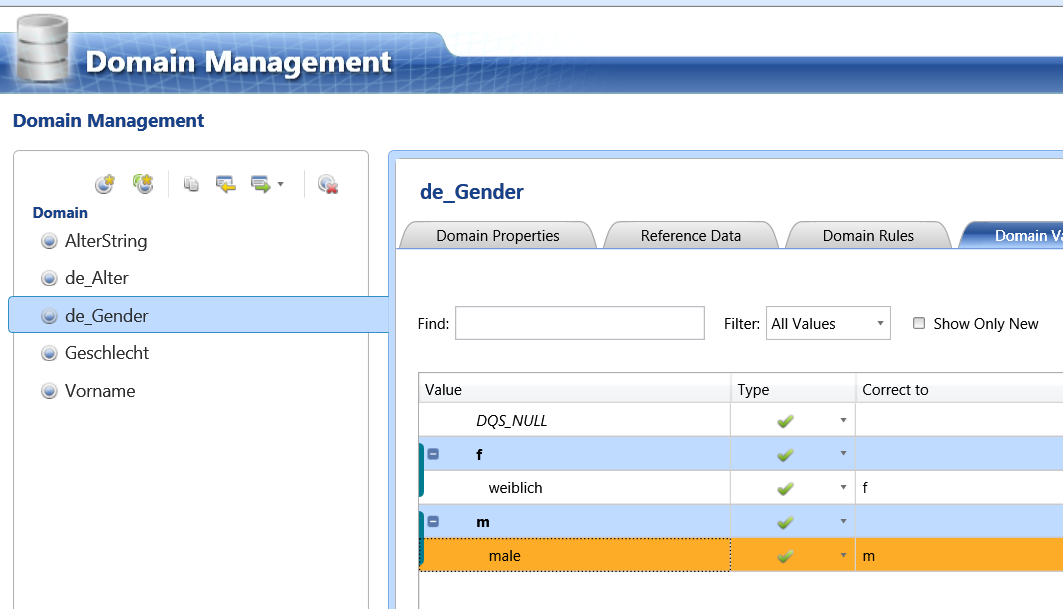
\includegraphics[width=0.80\textwidth]{doku/Bilder/KnowledgeGender.PNG}
	\caption{Dom�n Geschlecht mit Werten}
	\label{fig:KnowledgeGender}
\end{figure}

Die Bereinigung der Daten kann dann im SISS vorgenommen werden, wie es in Abbildung \ref{fig:SISS_DQS_Task} gezeigt ist. Der Task an sich ist recht sch�n. Man kann die Dom�ne zu einer Spalte angeben  und alle Regelen, die in der Kowledgebase verf�gbar sind werden angewendet. Als Ergebnis erh�lt man dann korrigierte oder aussortierte Daten, wie in Abbildung \ref{fig:DQS_Result} zu sehen ist.\footnote{In meinem Beispiel hat die Abbildung von Geschlecht m�nnlich nicht funktioniert und es wurde die ID der Spalte verwendet. Ich konnte nicht nachvollziehen warum das so ist.}

\begin{figure}
	\centering
		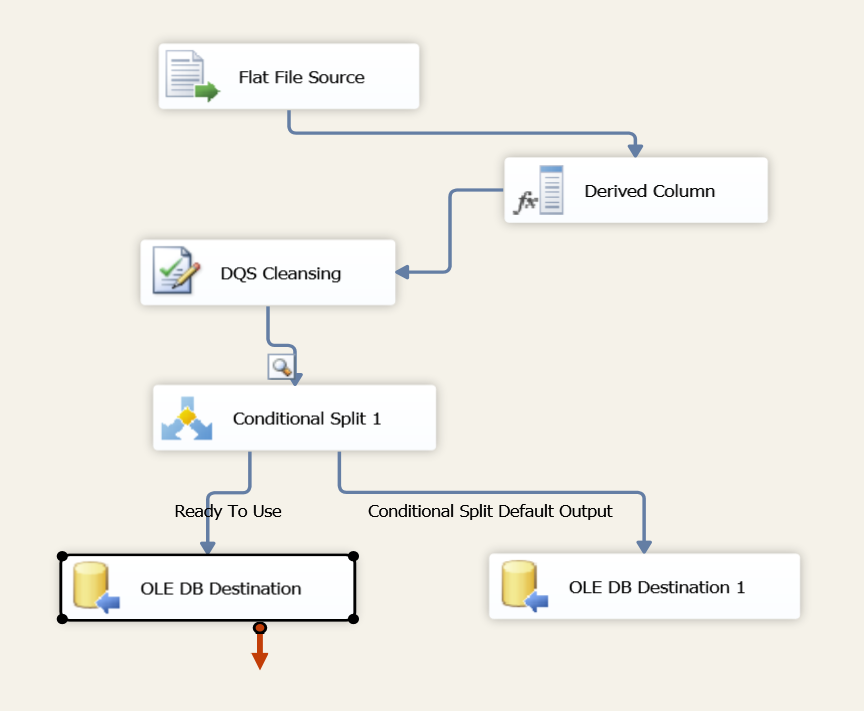
\includegraphics[width=1.00\textwidth]{doku/Bilder/SISS_DQS_Task.PNG}
	\caption{DQS Task in SISS}
	\label{fig:SISS_DQS_Task}
\end{figure}

\begin{figure}
	\centering
		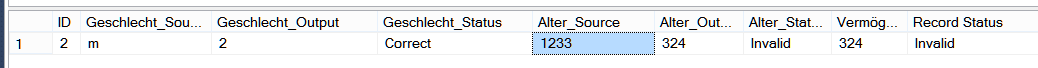
\includegraphics[width=1.00\textwidth]{doku/Bilder/DQS_Result.PNG}
	\caption{DQS Ergebins, invalide Daten}
	\label{fig:DQS_Result}
\end{figure}
